\documentclass[12pt]{scrbook}

\setkomafont{author}{\scshape}
\linespread{1}
\usepackage[margin=1in]{geometry} % 1 inch margins all around
\usepackage{graphicx} 
\graphicspath{ {../} }
\renewcommand\thesection{\arabic{section}}

\title{ECE656 Project Report}
\subtitle{Finding spam comments within the Yelp dataset}
\date{March 2018}
\author{Josh Reid\thanks{University of Waterloo}
\and Vincent Weng\footnotemark[1]}

\begin{document}
\maketitle
\section{Introduction}
Every year Yelp releases their extensive dataset to the public to analyse and try to find interesting
trends or draw new conclusions about their users or businesses listed on there.
This provides us an ideal dataset to study and analyse for ECE656 since it is such a large and diverse
dataset it means that there are several different conclusions that can be found and some potential
irregularities in their database structure that we can improve upon.
This report is broken up into two different sections, in the first section we analyse the structure
of the dataset to create an E-R diagram outlining the relation between all of the tables and drawing
their connections in a graphical, flow chart type visual representation.

Next we clean the data by performing sanity checks on the data to ensure that the data entered in the
tables makes logical sense and doesn't contain any erroneous entries.

After determining the sanity checks to be performed we determine which indices should be added to the
dataset to allow for efficient querying of the data to perform these sanity checks and to run the queries
required to perform the analysis required to draw our conclusion.

Finally now that the data is cleaned of any erroneous data and sufficiently indexed the analysis can
begin to begin determining what knowledge or trends can be inferred from the dataset.
For our report we analyse factors that increase the chance for a review to be spam or paid for to
either raise or lower a business' rating.
This includes looking at how long a user too between creating their account and leaving a review as
spammers will generally create many accounts and leave a positive or negative review immediately and then
leave the account dormant.
We then validated this correlation against the dataset and found...

In the second section of the report we created accounts for different levels of users who will
potentially need to use this database. The different user types accounted for includes:
\begin{enumerate}
  \item{A casual user who uses the application to browse search results. These users do not need
	to have an account; hence, they cannot submit reviews}
  \item{Critiques that use the application to browse results just like the casual user, but they also
	leave reviews for places they visit. A logged in user should only be provided enough privileges
	to write the review}
  \item{Business analysts can use the application to produce sales reports and may want to do
	special data mining and analysis. They cannot perform IUD (Insert/Update/Delete) operations
	on the database but should have access to creating extra views on the database
	schema}
  \item{Developers working with this database are able to create new tables and perform data
	cleaning and indexing. They are allowed to perform IUD operations on the database}
  \item{The database admin who has full access over the database}
\end{enumerate}

\section{Part 1}
\subsection{E-R Diagram}
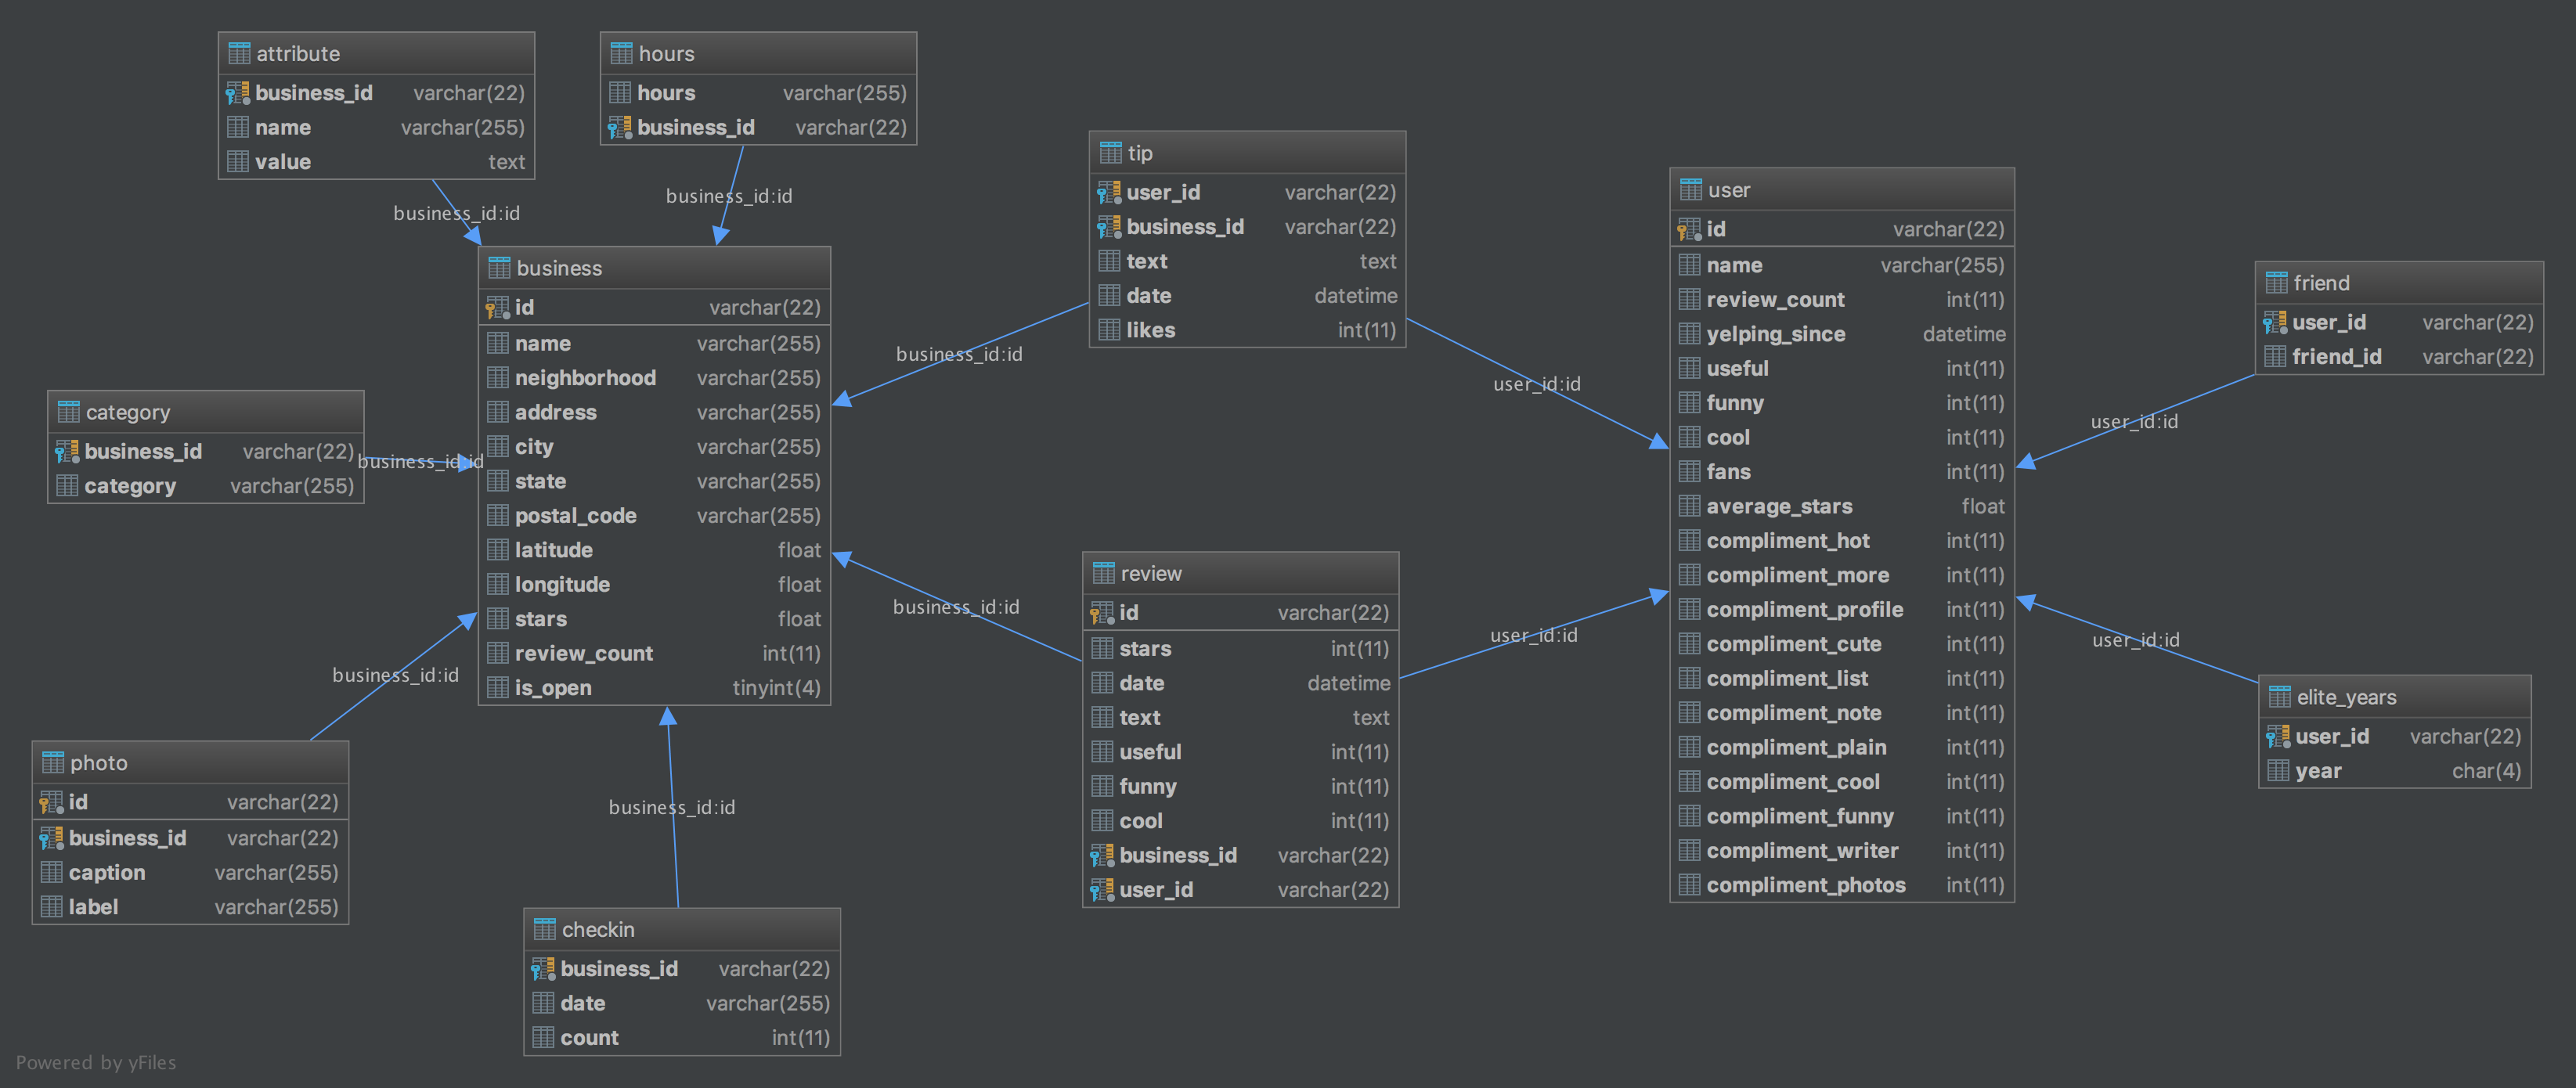
\includegraphics[width=\textwidth]{ER_Diagram}
\subsection{Data Cleaning}

\subsection{Data Analysis}

\subsubsection{Methods}

\subsubsection{Results}

\subsubsection{Graphs}

\subsection{Data Indexing}

\section{Part 2}
\subsection{Database Account Creation}

\end{document}
